\documentclass[../main.tex]{subfiles}
\graphicspath{{\subfix{../Images/}}}

\begin{document}

\chapter{Chapter 7. Environment Mapping Techniques}

This chapter explains environment mapping and presents several applications of the technique. The chapter has the following four sections:

\begin{itemize}
\item \textbf{"Environment Mapping"} introduces the technique and explains its key assumptions and limitations.
\item \textbf{"Reflective Environment Mapping"} explains the physics of reflection and how to simulate reflective materials with environment mapping.
\item \textbf{"Refractive Environment Mapping"} describes Snell's Law and shows how to use environment maps to implement an effect that approximates refraction.
\item \textbf{"The Fresnel Effect and Chromatic Dispersion"} combines reflection, refraction, the Fresnel effect, and the chromatic properties of light to produce a more complex effect called chromatic dispersion.
\end{itemize}

\section{7.1 Environment Mapping}

The preceding chapters showed some basic shading techniques. By now, you know how to light, transform, texture, and animate objects with Cg. However, your renderings are probably not quite what you envisioned. The next few chapters describe a few simple techniques that can dramatically improve your images.

This chapter presents several techniques based on \textit{environment mapping}. Environment mapping simulates an object reflecting its surroundings. In its simplest form, environment mapping gives rendered objects a chrome-like appearance.

Environment mapping assumes that an object's environment (that is, everything surrounding it) is infinitely distant from the object and, therefore, can be encoded in an omnidirectional image known as an environment map.

\subsection{7.1.1 Cube Map Textures}

All recent GPUs support a type of texture known as a \textit{cube map}. A cube map consists of not one, but six square texture images that fit together like the faces of a cube. Together, these six images form an omnidirectional image that we use to encode environment maps. Figure \ref{fig:7-1} shows an example of a cube map that captures an environment consisting of a cloudy sky and foggy mountainous terrain.

\begin{figure}
    \centering
    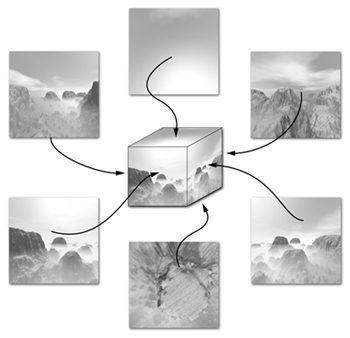
\includegraphics[width=1\linewidth]{fig7_1.jpg}
    \caption{Figure 7-1 Texture Images for a Cube Map}
    \label{fig:7-1}
\end{figure}

A 2D texture maps a 2D texture coordinate set to a color in a single texture image. In contrast, you access a cube map texture with a three-component texture coordinate set that represents a 3D direction vector.

Think of this vector as a ray originating from the center of the cube. As the ray shoots outward, it will intersect one of the six cube map faces. The result of a cube map texture access is the filtered color at that point of intersection with one of the six texture images.

Cube map textures are ideal for environment mapping. Each face of the cube map encodes one-sixth of the panoramic environment around an object. A cube map texture provides a quick way to determine what the object centered within that environment would "see" in any particular direction.

\subsection{7.1.2 Generating Cube Maps}

To generate a cube map, replace the object you want to put reflections on with a camera at the object's position and take snapshots in six directions (positive \textit{x}, negative \textit{x}, positive \textit{y}, negative \textit{y}, positive \textit{z}, and negative \textit{z}). Each snapshot should have a 90-degree field of view and a square aspect ratio, so that the six cube faces seam up tightly—with no gaps or overlap—to create an omnidirectional panorama. Use these images as the six faces of your cube map.

You can either render the six views with a computer, or capture an actual environment with a set of photographs and then warp them together to create an environment map. The electronic material that supplements this book contains pregenerated cube maps that you can use as well.

\subsection{7.1.3 The Environment Mapping Concept}

When you look at a highly reflective object such as a chrome sphere, what you see is not the object itself but how the object reflects its environment. When you gaze at some point on a highly reflective surface, the surface at that point reflects the \textit{view ray}—that is, the ray that travels from your eye to the point on the surface—into the environment. The characteristics of the reflected ray depend on the original view ray and on the surface normal at the point where the view ray reaches the surface. What you see is not the surface itself but what the environment looks like in the direction of the reflected ray.

When you use a cube map to encode what the environment looks like in all directions, rendering a point on a reflective surface is a matter of computing the reflected view direction for that point on the surface. Then you can access the cube map, based on the reflected view direction, to determine the color of the environment for the point on the surface.

\subsection{7.1.4 Computing Reflection Vectors}

Figure \ref{fig:7-2} illustrates an object, an eye position, and a cube map texture that captures the environment surrounding the object. Because Figure 7-2 is, of course, depicting a 3D scene in 2D, the object is shown as a trapezoid and the environment is shown as the surrounding square, rather than an actual cube

\begin{figure}
    \centering
    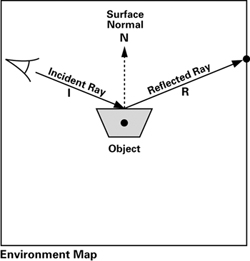
\includegraphics[width=0.75\linewidth]{fig7_2.jpg}
    \caption{Figure 7-2 Environment Mapping}
    \label{fig:7-2}
\end{figure}

The vector \textit{I}—called the \textit{incident ray}—goes from the eye to the object's surface. When \textit{I} reaches the surface, it is reflected in the direction \textit{R} based on the surface normal \textit{N}. This second ray is the \textit{reflected ray}. Figure \ref{fig:7-3} shows the geometry of the situation.

\begin{figure}
    \centering
    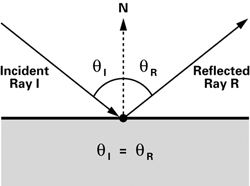
\includegraphics[width=0.5\linewidth]{fig7_3.jpg}
    \caption{Figure 7-3 Calculating the Reflected Ray}
    \label{fig:7-3}
\end{figure}

The angle of incidence ($\theta_I$) is the same as the angle of reflection ($\theta_R $) for a perfect reflector such as a mirror. You can compute the reflected vector \textit{R} in terms of the vectors \textit{I} and \textit{N} with Equation 7-1.

\FloatBarrier
\begin{equationcaption}
$
R = I - 2N(N \cdot I)
$
\caption{Equation 7-1 Vector Reflection}
\end{equationcaption}
\FloatBarrier

Calculating a reflected vector is a common operation in computer graphics, so Cg provides the \textbf{reflect} Standard Library function. This function takes in the incident vector and the surface normal and returns the reflected vector.

\FloatBarrier
\begin{table}
\centering
\begin{tabular}{ p{3cm} p{10cm}  } 
\hline
\textbf{reflect(I, N)} & Returns the reflected vector for the incident ray \textbf{I} and the surface normal \textbf{N}. The vector \textbf{N} should be normalized. The reflected vector's length is equal to the length of \textbf{I}. This function is valid only for three-component vectors. \\
\hline
\end{tabular}
\end{table}
\FloatBarrier

Though you are better off using the Cg Standard Library routine because of its efficiency, the straightforward implementation of \textbf{reflect} is as follows:

\FloatBarrier
\begin{lstlisting}
float3 reflect (float3  I, float3 N)
{
  return I - 2.0 * N * dot(N, I);
}
\end{lstlisting}
\FloatBarrier

We will be putting the \textbf{reflect} function to work later.

\subsection{7.1.5 Assumptions for Environment Mapping}

The preceding discussion mentioned that environment mapping assumes that the environment is infinitely distant from the object. Now we explore the implications of this assumption.

The reason for the assumption is that environment maps are accessed solely based on a 3D direction. Environment mapping has no allowance for variations in position to affect the reflected appearance of surfaces. If everything in the environment is sufficiently far away from the surface, then this assumption is approximately true.

In practice, the visual artifacts that result when the environment is not sufficiently distant typically go completely unnoticed. Reflections, particularly on curved surfaces, are subtle enough that most people fail to notice when a reflection is not physically accurate. As long as reflections match the coarse coloration of the environment and change appropriately with the curvature of the surface, surfaces rendered with environment mapping appear believable.

You'll be surprised at what you can get away with.

Ideally, every environment-mapped object in a scene should have its own environment map. In practice, objects can often share environment maps with no one noticing.

In theory, you should regenerate an environment map when objects in the environment move or when the reflective object using the environment map moves significantly relative to the environment. In practice, convincing reflections are possible with static environment maps.

With an environment map, an object can reflect only the environment; it cannot reflect itself. Similarly, do not expect multiple reflections, such as when two shiny objects reflect each other. Because an environment-mapped object can reflect only its environment and not itself, environment mapping works best on convex or mostly convex objects—rather than more concave objects.

Because environment mapping depends solely on direction and not on position, it works poorly on flat reflective surfaces such as mirrors, where the reflections depend heavily on position. In contrast, environment mapping works best on curved surfaces.

\section{7.2 Reflective Environment Mapping}

Let's start with the most common use of environment mapping: creating a chrome-like reflective object. This is the bare-bones application of the technique, yet it already produces nice results, as shown in Figure \ref{fig:7-4}.

\begin{figure}
    \centering
    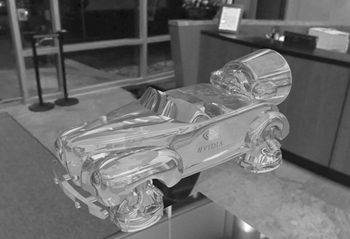
\includegraphics[width=1\linewidth]{fig7_4.jpg}
    \caption{Figure 7-4 Reflective Environment Mapping}
    \label{fig:7-4}
\end{figure}

In this example, the vertex program computes the incident and reflected rays. It then passes the reflected ray to the fragment program, which looks up the environment map and uses it to add a reflection to the fragment's final color. To make things more interesting, and to make our example more like a real application, we blend the reflection with a decal texture. A uniform parameter called \textbf{reflectivity} allows the application to control how reflective the material is.

You might wonder why we don't use the fragment program to calculate the reflection vector. A reflection vector computed per-fragment by the fragment program would deliver higher image quality, but it wouldn't work on basic fragment profiles. Therefore, we leave the per-fragment implementation as an exercise for you. Later in this chapter, we discuss the trade-offs and implications of using the vertex program versus using the fragment program.

\subsection{7.2.1 Application-Specified Parameters}

Table \ref{table:7-1} lists the data that the application needs to provide to the graphics pipeline.

\begin{table}
\centering
\begin{tabular}{ p{7cm} p{3cm} p{3cm} } 

Parameter & Variable Name & Type \\
\hline

\multicolumn{3}{p{10cm}}{\textbf{VERTEX PROGRAM VARYING PARAMETERS}}\\

Object-space vertex position & \textbf{position} & \textbf{float4} \\
Object-space vertex normal & \textbf{normal} & \textbf{float3} \\
Texture coordinates & \textbf{texCoord} & \textbf{float2} \\

\hline

\multicolumn{3}{p{10cm}}{\textbf{VERTEX PROGRAM UNIFORM PARAMETERS}}\\

Concatenated modelview and projection matrices & \textbf{modelViewProj} & \textbf{float4x4} \\
Eye position (in world space) & \textbf{eyePositionW} & \textbf{float3} \\
Object space to world space transform & \textbf{modelToWorld} & \textbf{float4x4} \\

\hline

\multicolumn{3}{p{10cm}}{\textbf{FRAGMENT PROGRAM UNIFORM PARAMETERS}}\\

Decal texture & \textbf{decalMap} & \textbf{sampler2D} \\
Environment map & \textbf{environmentMap} & \textbf{samplerCUBE} \\
Reflectivity & \textbf{reflectivity} &  \textbf{float} \\

\hline

\end{tabular}

\caption{Table 7-1. Application-Specified Parameters for Per-Vertex Environment Mapping}
\label{table:7-1}
\end{table}

\subsection{7.2.2 The Vertex Program}

Example 7-1 gives the vertex program that performs the per-vertex reflection vector computation for environment mapping.

\FloatBarrier
\begin{lstlisting}[caption=Example 7-1. The \textbf{C7E1v_reflection} Vertex Program]
void  C7E1v_reflection(float4  position : POSITION,
                       float2 texCoord : TEXCOORD0,
                       float3 normal : NORMAL,

                   out float4 oPosition : POSITION,
                   out float2 oTexCoord : TEXCOORD0,
                   out float3 R         : TEXCOORD1,

               uniform float3   eyePositionW,
               uniform float4x4 modelViewProj,
               uniform float4x4 modelToWorld)
{
  oPosition = mul(modelViewProj, position);
  oTexCoord = texCoord;

  // Compute position and normal in world space
  float3 positionW = mul(modelToWorld, position).xyz;
  float3 N = mul((float3x3)modelToWorld, normal);
  N = normalize(N);

  // Compute the incident and reflected vectors
  float3 I = positionW - eyePositionW;
  R = reflect(I, N);
}
\end{lstlisting}
\FloatBarrier

\subsection*{Basic Operations}

The vertex program starts with the mundane operations: transforming the position into clip space and passing through the texture coordinate set for the decal texture.

\FloatBarrier
\begin{lstlisting}
   oPosition = mul(modelViewProj, position);
   oTexCoord = texCoord;
\end{lstlisting}
\FloatBarrier

\subsection*{Transforming the Vectors into World Space}

Environment maps are typically oriented relative to world space, so you need to calculate the reflection vector in world space (or whatever coordinate system orients the environment map). To do that, you must transform the rest of the vertex data into world space. In particular, you need to transform the vertex position and normal by multiplying them by the \textbf{modelToWorld} matrix:

\FloatBarrier
\begin{lstlisting}
  float3 positionW = mul(modelToWorld, position).xyz;
  float3 N = mul((float3x3)modelToWorld, normal);
\end{lstlisting}
\FloatBarrier
  
The \textbf{modelToWorld} matrix is of type \textbf{float4x4}, but we require only the upper 3x3 section of the matrix when transforming a normal. Cg allows you to cast larger matrices to smaller matrices, as in the previous code. When you cast a larger matrix to a smaller matrix type, such as a \textbf{float4x4} matrix cast to a \textbf{float3x3} matrix, the upper left portion of the larger matrix fills in the matrix of the smaller type. For example, if you had a \textbf{float4x4} matrix \textit{M}:

$
M = \begin{bmatrix}
1.0 & 2.0 & 3.0 & 4.0 \\
5.0 & 6.0 & 7.0 & 8.0 \\
9.0 & 10.0 & 11.0 & 12.0 \\
13.0 & 14.0 & 15.0 & 16.0 \\
\end{bmatrix}
$

and you cast it to a \textbf{float3x3} matrix, you would end up with the matrix \textit{N}:

$
N = \begin{bmatrix}
1.0 & 2.0 & 3.0 \\
5.0 & 6.0 & 7.0 \\
9.0 & 10.0 & 11.0 \\
\end{bmatrix}
$

\begin{framed}
Advanced Topic

Recall from Chapter 4 (Section 4.1.3) that the modeling transform converts object-space coordinates to world-space coordinates. In this example, we assume that the modeling transform is \textit{affine} (rather than projective) and uniform in its scaling (rather than nonuniformly scaling \textit{x}, \textit{y}, and \textit{z}). We also assume that the \textit{w} component of \textbf{position} is 1, even \textbf{though} position is defined to be a \textbf{float4} in the prototype for \textbf{C7E1v_reflection}.

These assumptions are commonly true, but if they do not hold for your case, here is what you need to do.

If the modeling transform scales positions nonuniformly, you must multiply \textbf{normal} by the inverse transpose of the modeling matrix (\textbf{modelToWorldInvTrans}), rather than simply by \textbf{modelToWorld}. That is:

\FloatBarrier
\begin{lstlisting}
   float3  N = mul ((float3x3)modelToWorldInvTrans, normal);
\end{lstlisting}
\FloatBarrier
   
If the modeling transform is projective or the \textit{w} component of the object-space \textbf{position} is not 1, you must divide \textbf{positionW} by its \textit{w} component. That is:

\FloatBarrier
\begin{lstlisting}
   positionW /= positionW.w;
\end{lstlisting}
\FloatBarrier

The \textbf{/=} operator is an assignment operator, like the one in C and C++, which in this case divides \textbf{positionW} by \textbf{positionW.w} and then assigns the result to \textbf{positionW}.
\end{framed}

\subsection*{Normalizing the Normal}

The vertex normal needs to be normalized:

\FloatBarrier
\begin{lstlisting}
   N = normalize(N);
\end{lstlisting}
\FloatBarrier

\begin{framed}
Advanced Topic

In certain cases, we can skip this \textbf{normalize} function call. If we know that the upper 3x3 portion of the \textbf{modelToWorld} matrix causes no nonuniform scaling \textit{and} the object-space normal parameter is guaranteed to be already normalized, the \textbf{normalize} call is unnecessary.
\end{framed}

\subsection*{Calculating the Incident Vector}

The incident vector is the opposite of the view vector used in Chapter 5 for specular lighting. The \textit{incident vector} is the vector from the eye to the vertex (whereas the view vector is from the vertex to the eye). With the world-space eye position (\textbf{eyePositionW}) available as a uniform parameter and the world-space vertex position (\textbf{positionW}) available from the previous step, calculating the incident vector is a simple subtraction:

\FloatBarrier
\begin{lstlisting}
   float3 I = positionW - eyePositionW;
\end{lstlisting}
\FloatBarrier
   
\subsection*{Calculating the Reflection Vector}

You now have the vectors you need—the position and normal, both in world space—so you can calculate the reflection vector:

\FloatBarrier
\begin{lstlisting}
   float3 R = reflect(I, N);
\end{lstlisting}
\FloatBarrier
   
Next, the program outputs the reflected world-space vector \textbf{R} as a three-component texture coordinate set. The fragment program example that follows will use this texture coordinate set to access a cube map texture containing an environment map.

\subsection*{Normalizing Vectors}

You might be wondering why we did not normalize \textbf{I} or \textbf{R}. Normalization is not needed here because the reflected vector is used to query a cube map. The direction of the reflected vector is all that matters when accessing a cube map. Regardless of its length, the reflected ray will intersect the cube map at exactly the same location.

And because the \textbf{reflect} function outputs a reflected vector that has the same length as the incident vector as long as \textbf{N} is normalized, the incident vector's length doesn't matter either in this case.

There is one more reason not to normalize \textbf{R}. The rasterizer interpolates \textbf{R} prior to use by the fragment program in the next example. This interpolation is more accurate if the per-vertex reflection vector is not normalized.

\subsection{7.2.3 The Fragment Program}

Example 7-2 shows a fragment program that is quite short, because the \textbf{C7E1v_reflection} vertex program already took care of the major calculations. All that's left are the cube map lookup and the final color calculation.

\FloatBarrier
\begin{lstlisting}[caption=Example 7-2. The \textbf{C7E2f_reflection} Fragment Program]
void  C7E2f_reflection(float2 texCoord : TEXCOORD0,
                       float3 R        : TEXCOORD1,
                   out float4 color : COLOR,

               uniform float reflectivity,
               uniform sampler2D decalMap,
               uniform samplerCUBE environmentMap)
{
   // Fetch reflected environment color
   float4 reflectedColor = texCUBE(environmentMap, R);

   // Fetch the decal base color
   float4 decalColor = tex2D(decalMap, texCoord);

   color = lerp(decalColor, reflectedColor, reflectivity);
}
\end{lstlisting}
\FloatBarrier

The fragment program receives the interpolated reflected vector that it uses to obtain the reflected color from the environment map:

\FloatBarrier
\begin{lstlisting}
   float4  reflectedColor = texCUBE(environmentMap, R);
\end{lstlisting}
\FloatBarrier
   
Notice the new texture lookup function \textbf{texCUBE}. This function is used specifically for accessing cube maps, and so it interprets the second parameter (which is a three-component texture coordinate set) as a direction.

At this point, you could assign \textbf{reflectedColor} to \textbf{color}, making the rendered object completely reflective. However, no real material is a perfect reflector, so to make things more interesting, the program adds a decal texture lookup, and then mixes the decal color with the reflected color:

\FloatBarrier
\begin{lstlisting}
   float4  decalColor = tex2D(decalMap, texCoord);
   color = lerp(decalColor, reflectedColor, reflectivity);
\end{lstlisting}
\FloatBarrier
   
The \textbf{lerp} function performs linear interpolation, as you have seen before in Section 3.3.5. The parameters to \textbf{lerp} are \textbf{decalColor}, \textbf{reflectedColor}, and \textbf{reflectivity}. So, when \textbf{reflectivity} is 0, your program writes out just the decal color and shows no reflection. In contrast, when \textbf{reflectivity} is 1, the program writes out just the reflected color, producing a completely reflective, chrome-like appearance. Intermediate values of \textbf{reflectivity} result in a decaled model that has some reflective qualities.

\subsection{7.2.4 Control Maps}

\begin{framed}
Advanced Topic

In this example, \textbf{reflectivity} is a uniform parameter. The assumption is that each piece of geometry in the scene has the same reflectivity over its entire surface. But this doesn't necessarily have to be the case! You can create more interesting effects by encoding reflectivity in a texture. This approach allows you to vary the amount of reflectivity at each fragment, which makes it easy to create objects with both reflective and nonreflective parts.

Because the idea of using a texture to control shading parameters is so powerful, we call such a texture a \textit{control map}. Control maps are especially important because they leverage the GPU's efficient texture manipulation capabilities. In addition, control maps give artists increased control over effects without having to have a deep understanding of the underlying programs. For example, an artist could paint a "reflectivity map" without understanding how environment mapping works.

Control maps are an excellent way to add detail and complexity to almost any program.
\end{framed}

\subsection{7.2.5 Vertex Program vs. Fragment Program}

We mentioned previously that you could achieve higher image quality by using the fragment program (instead of the vertex program) to calculate the reflected vector. Why is this? It is for the same reason that per-fragment lighting looks better than per-vertex lighting.

As with specular lighting, the reflection vector for environment mapping varies in a nonlinear way from fragment to fragment. This means that linearly interpolated per-vertex values will be insufficient to capture accurately the variation in the reflection vector. In particular, subtle per-vertex artifacts tend to appear near the silhouettes of objects, where the reflection vector changes rapidly within each triangle. To obtain more accurate reflections, move the reflection vector calculation to the fragment program. This way, you explicitly calculate the reflection vector for each fragment instead of interpolating it.

Despite this additional accuracy, per-fragment environment mapping may not improve image quality enough to justify the additional expense. As explained earlier in the chapter, most people are unlikely to notice or appreciate the more correct reflections at glancing angles. Keep in mind that environment mapping does not generate physically correct reflections to begin with.

\section{7.3 Refractive Environment Mapping}

Now that you have learned how to implement basic environment mapping, you can use it to simulate some related physical phenomena. The techniques you will learn in the following sections illustrate how easy it is to put theory into practice when you are using a high-level language like Cg. The same techniques could be implemented without Cg, but they would require a great deal of assembly-level coding skill. As a result, the techniques and resulting image quality would be out of reach for most developers, even though the effects would be supported by the underlying graphics hardware.

In this section, you are going to learn how to implement refraction using a little physics and a little environment mapping. Figure \ref{fig:7-5} illustrates the effect you will be trying to achieve.

\begin{figure}
    \centering
    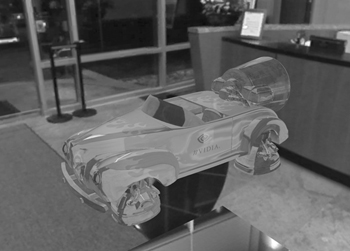
\includegraphics[width=1\linewidth]{fig7_5.jpg}
    \caption{Figure 7-5 Refractive Environment Mapping}
    \label{fig:7-5}
\end{figure}

\subsection{7.3.1 The Physics of Refraction}

When light passes through a boundary between two materials of different density (air and water, for example), the light's direction changes. This change in direction happens because light travels more slowly in denser materials (or \textit{media}, as materials are called in the context of refraction). For example, light travels quickly in air, but more slowly in water. The classic example of refraction is the "bend" that appears in a straw when you place it in a glass of water.

\subsection*{Snell's Law}

Snell's Law describes what happens to light at a boundary (or \textit{interface}, as such boundaries are called in the context of refraction) between two media, as shown in Figure \ref{fig:7-6}. The refracted vector is represented by \textit{T}, which stands for "transmitted." Snell's Law is expressed mathematically by Equation 7-2. The equation has four variables: the incident angle $\theta_I$, the refracted angle $\theta_T $, and an index of refraction for each medium, $\eta_1$ and $\eta_2$.

\begin{figure}
    \centering
    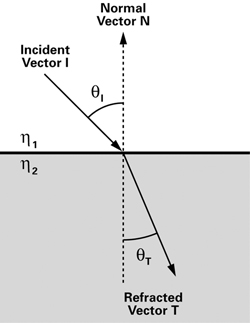
\includegraphics[width=0.5\linewidth]{fig7_6.jpg}
    \caption{Figure 7-6 Snell's Law}
    \label{fig:7-6}
\end{figure}

\FloatBarrier
\begin{equationcaption}
$
\eta_1sin\theta_I=\eta_2sin\theta_T
$
\caption{Equation 7-2 Snell's Law}
\end{equationcaption}
\FloatBarrier

A medium's index of refraction measures how the medium affects the speed of light. The higher the index of refraction for a medium, the slower light travels in it. Table \ref{table:7-2} lists a few common materials and their approximate indices of refraction. (The index of refraction for a material actually depends not only on the material, but also on the wavelength of the incoming light, but we ignore this complexity for the moment.)

\begin{table}
\centering
\begin{tabular}{ p{2cm} p{4cm} } 

Material & Index of Refraction \\
\hline

Vacuum & 1.0 \\
Air & 1.0003 \\
Water & 1.3333 \\
Glass & 1.5 \\
Plastic & 1.5 \\
Diamond & 2.417 \\

\hline

\end{tabular}

\caption{Table 7-2. Indices of Refraction}
\label{table:7-2}

\textbf{Notes}
Different types of glass have different indices of refraction, but 1.5 is a reasonable value for ordinary window glass. It is also a decent approximation for most plastics.

\end{table}

In this example, you will simulate refraction, as shown in Figure \ref{fig:7-7}. Each incident ray from the eye is refracted, and each refracted ray is used to look up the environment map (just as each reflected ray was used to look up the environment map in the reflection mapping example).

\begin{figure}
    \centering
    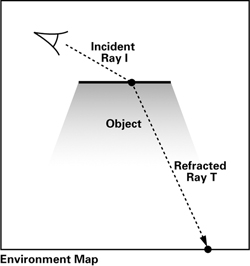
\includegraphics[width=0.5\linewidth]{fig7_7.jpg}
    \caption{Figure 7-7 Refraction into an Environment Map}
    \label{fig:7-7}
\end{figure}

Notice that we only simulate the first refracted ray. Figure \ref{fig:7-8} shows the difference for a simple object between our approach and a more accurate approach. The incident ray should really be refracted twice—once as it enters the object, and again as it leaves (as the vector $T'$). However, we do not simulate the second refraction, so we use $T$ instead of $T'$ as the transmitted ray. The two rays end up intersecting the environment in different locations (labeled A and B in Figure \ref{fig:7-8}). Fortunately, refraction is complicated enough that the resulting images are hard to distinguish in most cases. Especially for a casual viewer, it will be hard to tell that the generated refraction is not truly correct.

\begin{figure}
    \centering
    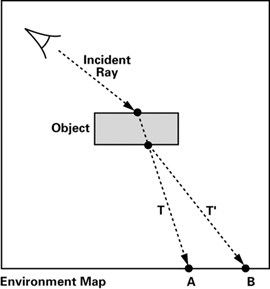
\includegraphics[width=0.5\linewidth]{fig7_8.jpg}
    \caption{Figure 7-8 Multiple Refractions vs. One Refraction}
    \label{fig:7-8}
\end{figure}

This type of simplification occurs routinely in real-time computer graphics. The thing to remember is that the result is what matters. If your images look convincing, it often doesn't matter that they might be physically inaccurate. In many cases, if you were to compute a complete physical simulation, your frame rate would drop significantly. This is why, from its early days, real-time computer graphics has focused on finding new, efficient techniques to make images look good. Of course, the goal is still to find techniques that are both accurate and fast, but in most cases, the programmer must still make an appropriate trade-off between accuracy and performance.

\subsection*{The Ratio of Indices of Refraction}

To calculate refraction, one of the key values you need is the ratio between the index of refraction of each medium. For the next example, the application needs to pass \textbf{etaRatio}, the ratio of indices of refraction of the two media, to the vertex program. Conventionally, the Greek letter $\eta$ ("eta") is used for a single material's index of refraction. However, the ratio of indices of refraction is more efficient in practice, because it saves the vertex program from having to calculate the ratio for each vertex (when it needs to be calculated only once per mesh).

\subsection{7.3.2 The Vertex Program}

Refraction is, in many ways, similar to reflection. In both cases, an incident ray hits a surface and something happens to it (it bounces off in the case of reflection, and it changes direction inside the surface in the case of refraction). These similarities hint that the Cg code for refraction is similar to the code for reflection. And indeed, it is.

The vertex program \textbf{C7E3v_refraction} in Example 7-3 for refraction needs to compute and output the refracted ray, rather than the reflected ray as in \textbf{C7E1v_reflection}. You do not need to apply Snell's Law yourself, because Cg has a \textbf{refract} function that will do it for you. Here is the function definition:

\FloatBarrier
\begin{table}
\centering
\begin{tabular}{ p{4cm} p{10cm}  } 
\hline
\textbf{refract(I, N, etaRatio)} & Given incident ray direction \textbf{I}, surface normal \textbf{N}, and relative index of refraction \textbf{etaRatio}, this function computes refraction vector \textbf{T}, as illustrated in Figure \ref{fig:7-6}. The vector \textbf{N} should be normalized. The refracted vector's length is equal to the length of \textbf{I}. \textbf{etaRatio} is the ratio of the index of refraction in the medium containing the incident ray to that of the medium being entered. This function is valid only for three-component vectors. \\
\hline
\end{tabular}
\end{table}
\FloatBarrier

Here is a sample implementation of the \textbf{refract} Standard Library routine:

\FloatBarrier
\begin{lstlisting}
float3 refract (float3  I, float3  N, float etaRatio)
{
  float cosI = dot(-I, N);
  float cosT2 = 1.0f - etaRatio * etaRatio *
                       (1.0f - cosI * cosI);
  float3 T = etaRatio * I +
             ((etaRatio * cosI - sqrt(abs(cosT2))) * N);
  return T * (float3)(cosT2 > 0);
}
\end{lstlisting}
\FloatBarrier

\FloatBarrier
\begin{lstlisting}[caption=Example 7-3. The \textbf{C7E3v_refraction} Vertex Program]
void  C7E3v_refraction(float4  position : POSITION,
                       float2  texCoord : TEXCOORD0,
                       float3  normal   : NORMAL,

                   out float4 oPosition : POSITION,
                   out float2 oTexCoord : TEXCOORD0,
                   out float3 T         : TEXCOORD1,

               uniform float etaRatio,
               uniform float3 eyePositionW,
               uniform float4x4 modelViewProj,
               uniform float4x4 modelToWorld)
{
  oPosition = mul(modelViewProj, position);
  oTexCoord = texCoord;

  // Compute position and normal in world space
  float3 positionW = mul(modelToWorld, position).xyz;
  float3 N = mul((float3x3)modelToWorld, normal);
  N = normalize(N);

  // Compute the incident and refracted vectors
  float3 I = normalize (positionW - eyePositionW);
  T = refract(I, N, etaRatio);
}
\end{lstlisting}
\FloatBarrier

\begin{framed}
Caution

When light passes from a dense medium to a less dense medium, the light can refract so much that total internal reflection occurs. For example, if you are under water in a pool and the surface of the water is smooth enough, the surface of the water will look like a mirror when viewed at a glancing angle. In this case, \textbf{cosT2} is less than or equal to zero and the \textbf{refract} routine returns a zero vector.
\end{framed}

The key difference between the earlier \textbf{C7E1v_reflection} example and the \textbf{C7E3v_refraction} example is the use of the \textbf{refract} function (rather than the \textbf{reflect} function) to calculate the refracted vector \textbf{T}. 

\subsection{7.3.3 The Fragment Program}

The fragment program does not have to be changed because its role remains the same: it looks up the environment map based on the incoming vector. The incoming vector is now the refracted vector instead of the reflected vector, but the fragment program still behaves exactly the same way that it did in the reflection mapping example. The fragment program looks up the environment map, mixes the result with the decal texture color, and returns the result. For correctness, the fragment program \textbf{C7E4f_refraction} in Example 7-4 renames \textbf{reflectedColor} to \textbf{refractedColor} and \textbf{reflectivity} to \textbf{transmittance}, but those are only cosmetic changes from the earlier \textbf{C7E2f_reflection} program.

\FloatBarrier
\begin{lstlisting}[caption=Example 7-4. The \textbf{C7E4f_refraction} Fragment Program]
void C7E4f_refraction(float2 texCoord : TEXCOORD0,
                      float3 T        : TEXCOORD1,

                  out float4 color : COLOR,

              uniform float       transmittance,
              uniform sampler2D   decalMap,
              uniform samplerCUBE environmentMap)
{
  // Fetch the decal base color
  float4 decalColor = tex2D(decalMap, texCoord);

  // Fetch refracted environment color
  float4 refractedColor = texCUBE(environmentMap, T);

  // Compute the final color
  color = lerp(decalColor, refractedColor, transmittance);
}
\end{lstlisting}
\FloatBarrier

\section{7.4 The Fresnel Effect and Chromatic Dispersion}

You now know how to implement reflection and refraction. The next example combines them and throws in a few other extensions. You will learn about two new effects: the Fresnel effect and chromatic dispersion.

\subsection{7.4.1 The Fresnel Effect}

In general, when light reaches an interface between two materials, some light reflects off the surface at the interface, and some refracts through the surface. This phenomenon is known as the \textit{Fresnel effect} (pronounced "freh-'nell"). The Fresnel equations describe how much light is reflected and how much is refracted. If you have ever wondered why you can see fish in a pond only when you're looking practically straight down, it's because of the Fresnel effect. At shallow angles, there is a lot of reflection and almost no refraction, so it is hard to see through the water's surface.

The Fresnel effect adds realism to your images, because it allows you to create objects that exhibit a mix of reflection and refraction, more like real-world objects.

The Fresnel equations, which quantify the Fresnel effect, are complicated. (You can learn more about them in most optics textbooks.) Once again, the idea here is to create images that look plausible, not necessarily to describe accurately the intricacies of the underlying physics. So, instead of using the equations themselves, we are going to use the empirical approximation in Equation 7-3, which gives good results with significantly less complication:

\FloatBarrier
\begin{equationcaption}
$
reflectionCoefficient = max(0,min(1,bias+scale*(1+I \cdot N)^{power}))
$
\caption{Equation 7-3 An Approximation of the Fresnel Equation}
\end{equationcaption}
\FloatBarrier

The concept underlying this equation is that when \textit{I} and \textit{N} are nearly coincident, the reflection coefficient should be 0 or nearly 0, indicating that most of the light should be refracted. As \textit{I} and \textit{N} diverge, the reflection coefficient should gradually increase and eventually abruptly increase (due to the exponentiation) to 1. When \textit{I} and \textit{N} are sufficiently divergent, almost all the light should be reflected, with little or none of it being refracted.

The range of the reflection coefficient is clamped to the range [0, 1], because we use the reflection coefficient to mix the reflected and refracted contributions according to the following formula (where $C$ stands for color):

$C_{Final} = reflectionCoefficient * C_{Reflected} + (1 - reflectionCoefficient) * C_{Refracted}$

\subsection{7.4.2 Chromatic Dispersion}

The earlier discussion of refraction was somewhat simplified. We mentioned that refraction depends on the surface normal, incident angle, and ratio of indices of refraction. In addition to these factors, the amount of refraction also depends on the wavelength of the incident light. For example, red light gets refracted more than blue light. This phenomenon is known as \textit{chromatic dispersion}, and it is what happens when white light enters a prism and emerges as a rainbow.

Figure \ref{fig:7-9} illustrates chromatic dispersion conceptually. The incident illumination (assumed to be white) is split into several refracted rays. You will simulate what happens to the red, green, and blue components of the light, because these are the standard components of colors in computer graphics. You will use the refracted red, green, and blue rays to look up into the environment map, just as you did for a single ray in the refraction example.

\begin{figure}
    \centering
    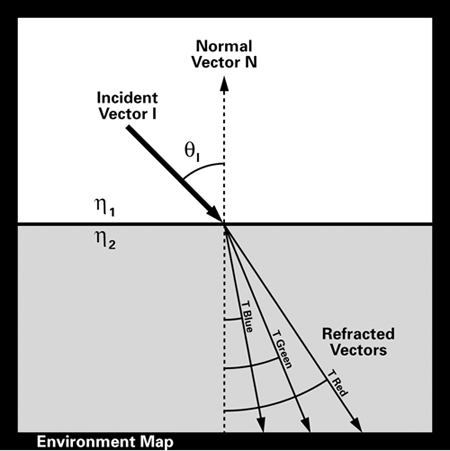
\includegraphics[width=0.75\linewidth]{fig7_9.jpg}
    \caption{Figure 7-9 Understanding Chromatic Dispersion}
    \label{fig:7-9}
\end{figure}

Keep in mind that real light is a band of wavelengths rather than three particular and discrete wavelengths. Still, this approximation is effective enough to be useful.

Combining the Fresnel effect with chromatic dispersion creates a rainbow effect, as if the rendered object were made of crystal, as shown in Figure \ref{fig:7-10}. Plate 11, in the book's center insert, shows this image in color.

\begin{figure}
    \centering
    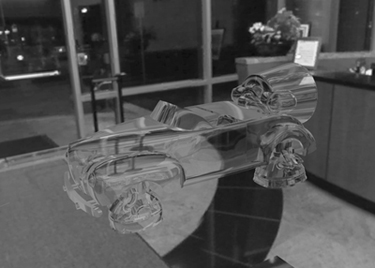
\includegraphics[width=1\linewidth]{fig7_10.jpg}
    \caption{Figure 7-10 The Fresnel Effect and Chromatic Dispersion}
    \label{fig:7-10}
\end{figure}

\subsection{7.4.3 Application-Specified Parameters}

Because we are now using a more complicated lighting model for our object's surface, the application needs to send extra uniform parameters to the vertex and fragment programs. These additional parameters are listed in Table \ref{table:7-3}.

\begin{table}
\centering
\begin{tabular}{ p{5cm} p{4cm} p{2cm}  } 

Parameter & Variable Name & Type \\
\hline

Ratio of indices of refraction for red, green, and blue light (packed into one \textbf{float3}) & \textbf{etaRatio} & \textbf{float3} \\
Fresnel power & \textbf{fresnelPower} & \textbf{float} \\
Fresnel scale & \textbf{fresnelScale} & \textbf{float} \\
Fresnel bias & \textbf{fresnelBias} & \textbf{float} \\

\hline

\end{tabular}

\caption{Table 7-3. The \textbf{C7E5v_dispersion} Program Parameters}
\label{table:7-3}

\end{table}

The \textbf{x}, \textbf{y}, and \textbf{z} components in \textbf{etaRatio}, respectively, store the ratio of indices of refraction for red, green, and blue light. The \textbf{fresnelPower}, \textbf{fresnelScale}, and \textbf{fresnelBias} variables provide a way to shape the function that we use to approximate the Fresnel equations. Together, all the application-specified parameters define the material properties of your object.

\subsection{7.4.4 The Vertex Program}

The \textbf{C7E5v_dispersion} vertex program in Example 7-5 calculates the reflected vector, along with red, green, and blue refracted vectors. In addition, you will use the approximation of Fresnel's formula to compute the reflection coefficient. All this information is then interpolated and received by the fragment program.

\subsection*{Calculating the Reflected Vector}

The reflected vector calculation stays the same:

\FloatBarrier
\begin{lstlisting}
   R = reflect(I, N);
\end{lstlisting}
\FloatBarrier
   
\subsection*{Calculating the Refracted Vectors}

You compute refracted vectors using an approach that is similar to the one that you used in the earlier refraction example. The difference is that now you have to calculate a refraction vector for each color component, instead of just one that applies equally to red, green, and blue:

\FloatBarrier
\begin{lstlisting}
   TRed   = refract(I, N, etaRatio.x);
   TGreen = refract(I, N, etaRatio.y);
   TBlue  = refract(I, N, etaRatio.z);
\end{lstlisting}
\FloatBarrier
   
Recall that the \textbf{x}, \textbf{y}, and \textbf{z} components in \textbf{etaRatio} respectively store the ratio of indices of refraction for red, green, and blue light.

\FloatBarrier
\begin{lstlisting}[caption=Example 7-5. The \textbf{C7E5v_dispersion} Vertex Program]
void C7E5v_dispersion(float4  position : POSITION,
                      float3  normal   : NORMAL,

                  out float4 oPosition         : POSITION,
                  out float  reflectionFactor  : COLOR,
                  out float3 R                 : TEXCOORD0,
                  out float3 TRed              : TEXCOORD1,
                  out float3 TGreen            : TEXCOORD2,
                  out float3 TBlue             : TEXCOORD3,

              uniform float fresnelBias,
              uniform float fresnelScale,
              uniform float fresnelPower,
              uniform float3 etaRatio,
              uniform float3 eyePositionW,
              uniform float4x4 modelViewProj,
              uniform float4x4 modelToWorld)
{
  oPosition = mul(modelViewProj, position);

  // Compute position and normal in world space
  float3 positionW = mul(modelToWorld, position).xyz;
  float3 N = mul((float3x3)modelToWorld, normal);
  N = normalize(N);

  // Compute the incident, reflected, and refracted vectors
  float3 I = positionW - eyePositionW;
  R = reflect(I, N);
  I = normalize(I);
  TRed   = refract(I, N, etaRatio.x);
  TGreen = refract(I, N, etaRatio.y);
  TBlue  = refract(I, N, etaRatio.z);

  // Compute the reflection factor
  reflectionFactor = fresnelBias +
                     fresnelScale * pow(1 + dot(I, N),
                                        fresnelPower);
}
\end{lstlisting}
\FloatBarrier

\subsection*{Calculating the Reflection Coefficient}

Translating Equation 7-3 into Cg code is straightforward. Use the \textbf{dot} and \textbf{pow} functions. The program outputs \textbf{reflectionFactor} as an interpolated color, as indicated by its associated \textbf{COLOR} semantic. Interpolated colors are automatically clamped to the range [0, 1], so there is no need to perform this clamping explicitly.

\FloatBarrier
\begin{lstlisting}
   reflectionFactor = fresnelBias +
                   fresnelScale * pow(1 + dot(I, N),
                                      fresnelPower);
\end{lstlisting}
\FloatBarrier

\subsection{7.4.5 The Fragment Program}

The \textbf{C7E6f_dispersion} fragment program in Example 7-6 receives all the interpolated data for the reflected and refracted vectors, along with the reflection coefficient that is clamped to [0, 1]. The fragment program looks up the various reflected and refracted vectors in an environment map and blends the results appropriately. Notice that the program expects the same environment cube map texture for each of the four texture units. The application must bind the environment map to each of these four texture units, because the program is written to run on both basic and advanced fragment profiles. Recall that basic fragment profiles can only sample a given texture unit with that texture unit's corresponding texture coordinate set, so the environment map must be replicated. Advanced fragment profiles do not have this limitation, so a single \textbf{environmentMap} cube map sampler would suffice.

\subsection*{Performing the Texture Lookups}

First, the program performs four cube map lookups—one for the reflected color, and one for each component of the three refracted colors:

\FloatBarrier
\begin{lstlisting}
   // Fetch the reflected environment color
   float4 reflectedColor = texCUBE(environmentMap0, R);

   // Compute the refracted environment color
   float4 refractedColor;
   refractedColor.r = texCUBE(environmentMap1, TRed).r;
   refractedColor.g = texCUBE(environmentMap2, TGreen).g;
   refractedColor.b = texCUBE(environmentMap3, TBlue).b;
\end{lstlisting}
\FloatBarrier

For each of the three refracted texture lookups, the program uses swizzling to extract only the matching color component. That is, you extract the red component of the texture value sampled at \textbf{TRed}, the green component of the texture value sampled at \textbf{TGreen}, and the blue component of the texture value sampled at \textbf{TBlue}. The program then combines the respective \textit{r}, \textit{g}, and \textit{b} components of \textbf{refractedColor}.

\FloatBarrier
\begin{lstlisting}[caption=Example 7-6. The \textbf{C7E6f_dispersion} Fragment Program]
void C7E6f_dispersion(float  reflectionFactor : COLOR,
                      float3 R                : TEXCOORD0,
                      float3 TRed             : TEXCOORD1,
                      float3 TGreen           : TEXCOORD2,
                      float3 TBlue            : TEXCOORD3,

                 out float4 color : COLOR,

             uniform samplerCUBE environmentMap0,
             uniform samplerCUBE environmentMap1,
             uniform samplerCUBE environmentMap2,
             uniform samplerCUBE environmentMap3)
{
  // Fetch the reflected environment color
  float4 reflectedColor = texCUBE(environmentMap0, R);

  // Compute the refracted environment color
  float4 refractedColor;
  refractedColor.r = texCUBE(environmentMap1, TRed).r;
  refractedColor.g = texCUBE(environmentMap2, TGreen).g;
  refractedColor.b = texCUBE(environmentMap3, TBlue).b;
  refractedColor.a = 1;

  // Compute the final color
  color = lerp(refractedColor,
               reflectedColor,
               reflectionFactor);
}
\end{lstlisting}
\FloatBarrier

\subsection*{Computing the Final Result}

Finally, the program blends the reflected and refracted colors according to the fraction given by the reflection factor:

\FloatBarrier
\begin{lstlisting}
color = lerp(refractedColor,
             reflectedColor,
             reflectionFactor);
\end{lstlisting}
\FloatBarrier

And there you have it: the Fresnel effect with chromatic dispersion.

\section{7.5 Exercises}

\begin{enumerate}

\item \textbf{Answer this:} What are the key assumptions behind environment mapping? For what situations does it break down?

\item \textbf{Try this yourself:} How would Figure \ref{fig:7-10} look if the value for the \textbf{etaRatio} index of refraction vector in \textbf{C7E5v_dispersion} were (1, 1, 1)?

\item \textbf{Try this yourself:} Try reimplementing the \textbf{C7E1v_reflection} vertex program to perform the reflection vector computation in object space and then transforming the resulting object-space reflection vector into world space.

\item \textbf{Answer this:} What is the Fresnel effect?

\item \textbf{Try this yourself:} When mipmapping is enabled, both OpenGL and Direct3D support a texture mapping feature known as texture \textit{level-of-detail} (LOD) bias. Texture LOD bias can be useful to avoid unnaturally crisp reflections. Modify one of this chapter's examples to provide a positive bias for the cube map texture used as the environment map. This creates blurry reflections.

\item \textbf{Answer this:} Prior to hardware support for cube map textures, a technique known as \textit{sphere mapping} was used to project 3D vectors onto a 2D texture. Research this technique and explain why everyone uses cube map textures now.

\end{enumerate}

\section{7.6 Further Reading}

Jim Blinn and Martin Newell introduced environment mapping in a 1976 paper titled "Texture and Reflection in Computer Generated Images," which appeared in the \textit{Communications of the ACM}.

Ned Greene published an important paper titled "Environment Mapping and Other Applications of World Projections," which appeared in a 1986 issue of \textit{IEEE Computer Graphics and Applications}. Greene proposed the idea of storing environment maps as cube maps.

RenderMan uses cube map textures for its environment mapping support. See \textit{The RenderMan Companion: A Programmer's Guide to Realistic Computer Graphics} (Addison-Wesley, 1989), by Steve Upstill, for more details.

Doug Voorhies and Jim Foran published a SIGGRAPH paper titled "Reflection Vector Shading Hardware" (ACM Press) in 1994. The paper proposed a dedicated hardware approach for computing per-fragment reflection vectors that were used to sample an environment map stored in a cube map texture.

OpenGL 1.3 and DirectX 7 introduced hardware support for cube map textures. The OpenGL 1.3 or later specification provides the mathematics for how texture coordinates map to particular cube faces.

Matthias Wloka's 2002 paper "Fresnel Reflection" (available on NVIDIA's Developer Web site, \textbf{developer.nvidia.com}) discusses the Fresnel effect in further detail. The paper explains various implementations and trade-offs between them.

\end{document}